\documentclass[a4paper,11pt]{article}
\usepackage[utf8]{inputenc}
\usepackage[T1]{fontenc}
\usepackage{amsmath,amssymb}
\usepackage[a4paper,left=2cm,right=2cm,top=3.6cm,bottom=2.3cm,headheight=1.1cm,headsep=0.6cm,footskip=1cm]{geometry}
\usepackage{xcolor}
\usepackage{tikz}
\usetikzlibrary{calc,arrows.meta,positioning,shapes.geometric}
\usepackage{fancyhdr}
\usepackage{lastpage}
\usepackage{tabularx}
\usepackage{array}
\usepackage[most]{tcolorbox}
\usepackage{enumitem}
\usepackage{needspace}

% ---------- palet merah dan merah muda ----------
\definecolor{redx}{HTML}{B3202F}
\definecolor{pinkx}{HTML}{E0457B}
\definecolor{maroon}{HTML}{7A1C2C}
\definecolor{softbg}{HTML}{FDF1F4}
\definecolor{salmon}{HTML}{E8836F}
\newcommand{\dis}{\displaystyle}
\newcommand{\sm}[1]{\left[\begin{smallmatrix}#1\end{smallmatrix}\right]}

\setlength{\parindent}{0pt}
\renewcommand{\arraystretch}{1.35}

\tikzset{
  ar/.style={-{Stealth[length=1.8mm]},thick,redx},
  box/.style={draw=redx,thick,rounded corners=3pt,fill=softbg,align=center,inner sep=4pt}
}

% ---------- header berwarna merah ----------
\pagestyle{fancy}
\fancyhf{}
\renewcommand{\headrulewidth}{0pt}
\fancyhead[L]{%
  \begin{tikzpicture}[remember picture,overlay]
    \fill[redx] ([yshift=-1.2cm]current page.north west) rectangle ([yshift=-3.15cm]current page.north east);
    \fill[pinkx] ([yshift=-3.15cm]current page.north west) rectangle ([yshift=-3.25cm]current page.north east);
  \end{tikzpicture}%
  \color{white}\bfseries\large Latihan Soal Transformasi Geometri}
\fancyhead[R]{\color{white}\small Diunduh dari website \textbf{Math1729}\ \,|\,\ 4 Oktober 2026}
\fancyfoot[L]{\small\color{redx}Math1729 --- Transformasi Geometri}
\fancyfoot[R]{\small\color{redx}Halaman \thepage\ dari \pageref{LastPage}}

% ---------- komponen ----------
\newcounter{no}
\newcommand{\bagian}[2]{\par\Needspace{6\baselineskip}\vspace{1.0em}\noindent
  \begin{tcolorbox}[colback=redx,colframe=redx,coltext=white,boxrule=0pt,arc=2pt,left=6pt,right=6pt,top=3pt,bottom=3pt]
  \textbf{#1}\hfill{\small #2}\end{tcolorbox}\setcounter{no}{0}\par\vspace{-0.3em}}
\newcommand{\tingkat}[2]{\par\Needspace{7\baselineskip}\vspace{0.6em}\noindent
  {\color{pinkx}\rule{3pt}{1.1em}}\ {\color{redx}\bfseries #1}\ {\small\color{gray}--- #2}\par\vspace{0.1em}}
\newcommand{\soal}[2]{\par\vspace{0.75em}\stepcounter{no}\noindent
  \begin{minipage}[t]{1.8em}\textbf{\theno.}\end{minipage}%
  \begin{minipage}[t]{\dimexpr\linewidth-1.8em\relax}#1\par\vspace{0.35em}#2\end{minipage}\par}
\newcommand{\poin}[1]{\hfill{\small\color{redx}[#1 poin]}}

% teks di kiri, gambar di kanan
\newcommand{\gbr}[2]{\noindent\begin{minipage}[t]{0.56\linewidth}#1\end{minipage}\hfill\raisebox{\ht\strutbox}{\begin{minipage}[t]{0.41\linewidth}\vspace{0pt}\centering#2\end{minipage}}}

% pilihan jawaban
\newcommand{\pil}[5]{\begin{tabularx}{\linewidth}{@{}*{5}{X}@{}}\textbf{A.}\;#1 & \textbf{B.}\;#2 & \textbf{C.}\;#3 & \textbf{D.}\;#4 & \textbf{E.}\;#5\end{tabularx}}
\newcommand{\pilx}[5]{\begin{tabularx}{\linewidth}{@{}*{3}{X}@{}}\textbf{A.}\;#1 & \textbf{B.}\;#2 & \textbf{C.}\;#3\\[10pt] \textbf{D.}\;#4 & \textbf{E.}\;#5 & \end{tabularx}}
% pilihan ganda kompleks (pilih semua yang benar)
\newcommand{\pilk}[5]{\begin{tabularx}{\linewidth}{@{}c@{\;}l@{\;}X@{}}$\square$&\textbf{A.}&#1\\[1pt]$\square$&\textbf{B.}&#2\\[1pt]$\square$&\textbf{C.}&#3\\[1pt]$\square$&\textbf{D.}&#4\\[1pt]$\square$&\textbf{E.}&#5\end{tabularx}}
% pilihan ganda kategori (Benar/Salah)
\newcommand{\kat}[4]{\begin{tabularx}{\linewidth}{@{}c@{\hspace{5pt}}X@{\hspace{6pt}}c@{\hspace{6pt}}c@{}}\hline\textbf{No}&\textbf{Pernyataan}&\textbf{Benar}&\textbf{Salah}\\\hline 1&#1&$\square$&$\square$\\\hline 2&#2&$\square$&$\square$\\\hline 3&#3&$\square$&$\square$\\\hline 4&#4&$\square$&$\square$\\\hline\end{tabularx}}
\newcommand{\jwb}{\hfill Jawaban: \rule{4.5cm}{0.4pt}}

% sumbu koordinat: \axg{xmin}{ymin}{xmax}{ymax}
\newcommand{\axg}[4]{%
  \draw[gray!30,very thin] (#1,#2) grid (#3,#4);
  \draw[->,thick,redx] (#1,0)--(#3+0.5,0) node[right,font=\scriptsize]{$x$};
  \draw[->,thick,redx] (0,#2)--(0,#4+0.5) node[above,font=\scriptsize]{$y$};
  \foreach \i in {#1,...,#3}{\ifnum\i=0\else\draw (\i,0.07)--(\i,-0.07) node[below,font=\tiny,inner sep=1pt,text=gray!60!black]{$\i$};\fi}
  \foreach \i in {#2,...,#4}{\ifnum\i=0\else\draw (0.07,\i)--(-0.07,\i) node[left,font=\tiny,inner sep=1pt,text=gray!60!black]{$\i$};\fi}}
% titik berlabel: \pnt{x}{y}{label}{posisi}
\newcommand{\pnt}[4]{\fill[maroon] (#1,#2) circle (1.5pt) node[#4,font=\scriptsize,inner sep=2pt]{$#3$};}

\begin{document}
\thispagestyle{fancy}

\begin{center}
  {\color{redx}\fontsize{22}{26}\selectfont\bfseries Latihan Soal Transformasi Geometri\par}
  \vspace{2pt}
  {\color{pinkx}\large Translasi, Refleksi, Rotasi, Dilatasi, Komposisi, Bayangan Garis, dan Matriks Transformasi\par}
\end{center}
\vspace{2pt}
\begin{tcolorbox}[colback=softbg,colframe=redx!40,boxrule=0.6pt,arc=3pt,left=8pt,right=8pt,top=5pt,bottom=5pt]
\noindent\textbf{Nama} : \rule{4.6cm}{0.4pt}\hfill\textbf{Kelas} : \rule{2.2cm}{0.4pt}\hfill\textbf{Skor} : \rule{2.2cm}{0.4pt}
\end{tcolorbox}
\vspace{2pt}
\begin{tcolorbox}[colback=white,colframe=pinkx,boxrule=0.8pt,arc=3pt,left=8pt,right=8pt,top=4pt,bottom=4pt,title={\bfseries Petunjuk Pengerjaan},coltitle=white,fonttitle=\small]
\small
\begin{enumerate}[leftmargin=1.4em,itemsep=1pt,topsep=1pt]
\item Soal terdiri atas \textbf{20 pilihan ganda} (5 mudah, 5 sedang, 5 sulit, 5 HOTS), \textbf{5 isian singkat} (2 sedang, 3 sulit), dan \textbf{5 uraian} (2 sedang, 2 sulit, 1 HOTS). Soal disusun berjenjang dari mudah sampai HOTS. Alokasi waktu yang disarankan: 120 menit.
\item Bentuk soal mengikuti pola asesmen terbaru (TKA dan UTBK-SNBT 2026): \textbf{pilihan ganda biasa} (satu jawaban benar); \textbf{pilihan ganda kompleks}, yaitu soal 5 dan 14, pilih \emph{semua} jawaban yang benar dengan memberi tanda pada kotak $\square$; \textbf{pilihan ganda kategori}, yaitu soal 10 dan 20, tentukan benar atau salah setiap pernyataan; \textbf{soal berstimulus}, yaitu soal 19 dan 20 yang memakai satu informasi bersama; serta \textbf{isian singkat}.
\item Skor: pilihan ganda 2 poin, isian singkat 4 poin, uraian 8 poin per soal (total 100 poin). Soal pilihan ganda kompleks dan kategori bernilai penuh hanya jika \emph{semua} bagian benar. Tidak ada pengurangan skor untuk jawaban salah.
\item Notasi: $P'$ bayangan titik $P$; $T\sm{a\\b}$ translasi; $R$ rotasi (sudut positif berlawanan arah jarum jam); $L$ luas. Pada komposisi $B\circ A$, transformasi $A$ dikerjakan lebih dahulu. Gambar tidak selalu digambar sesuai skala.
\item Kalkulator tidak diperkenankan. Jawaban bentuk akar dan pecahan tidak perlu didesimalkan.
\end{enumerate}
\end{tcolorbox}

% =====================================================================
\bagian{A. Pilihan Ganda}{20 soal $\times$ 2 poin = 40 poin. Pilih jawaban yang paling tepat sesuai bentuk soal.}

\tingkat{Tingkat Mudah}{soal 1 sampai 5}
\soal{Pada peta kota, menara pemancar di titik $A(-2,6)$ dipindahkan ke $A'(5,1)$ oleh suatu translasi $T$. Kantor pos di titik $B(3,-4)$ ikut dipindahkan oleh translasi $T$ yang sama. Koordinat bayangan kantor pos adalah \dots.}{\pil{$(-4,1)$}{$(10,1)$}{$(6,-9)$}{$(10,-9)$}{$(-4,-9)$}}
\soal{\gbr{Segitiga $ABC$ dengan $A(-3,3)$, $B(1,3)$, dan $C(-1,6)$ dicerminkan terhadap garis $y=2$ (garis putus-putus pada gambar). Koordinat bayangan titik $C$ adalah \dots.}{%
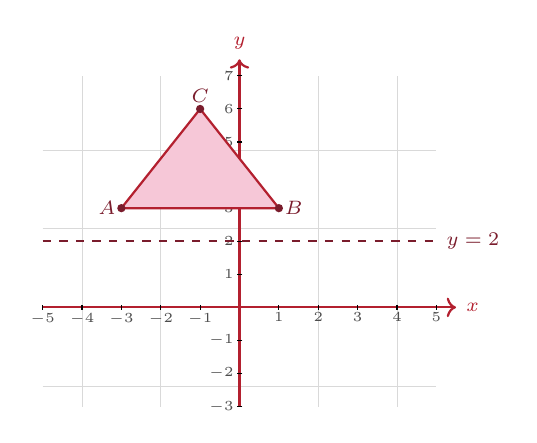
\begin{tikzpicture}[x=0.5cm,y=0.42cm]
\axg{-5}{-3}{5}{7}
\fill[pinkx!30] (-3,3)--(1,3)--(-1,6)--cycle;
\draw[redx,thick] (-3,3)--(1,3)--(-1,6)--cycle;
\draw[dashed,maroon,thick] (-5,2)--(5,2) node[right,font=\scriptsize]{$y=2$};
\pnt{-3}{3}{A}{left}\pnt{1}{3}{B}{right}\pnt{-1}{6}{C}{above}
\end{tikzpicture}}}{\pil{$(-1,-6)$}{$(-1,-4)$}{$(-1,-2)$}{$(-1,10)$}{$(5,6)$}}
\soal{Titik $Q(-3,5)$ pada layar sebuah permainan diputar sejauh $270^\circ$ berlawanan arah jarum jam dengan pusat $O(0,0)$. Koordinat bayangan $Q$ adalah \dots.}{\pil{$(-5,-3)$}{$(3,-5)$}{$(5,-3)$}{$(-3,-5)$}{$(5,3)$}}
\soal{Dilatasi berpusat di $O(0,0)$ memetakan titik $A(3,-2)$ ke $A'(-12,8)$. Bayangan titik $B(-1,5)$ oleh dilatasi yang sama adalah \dots.}{\pil{$(4,-20)$}{$(-4,20)$}{$(4,20)$}{$(-20,4)$}{$(20,-4)$}}
\soal{Pilih \emph{semua} transformasi berikut yang selalu mempertahankan luas bangun yang ditransformasikan.}{\pilk{Refleksi terhadap garis $y=-x$.}{Rotasi sebesar $135^\circ$ dengan pusat $(2,3)$.}{Dilatasi berpusat di $O$ dengan faktor $2$.}{Translasi oleh $\sm{-5\\8}$.}{Dilatasi berpusat di $(1,1)$ dengan faktor $-1$.}}

\tingkat{Tingkat Sedang}{soal 6 sampai 10}
\soal{Matriks $M=\begin{bmatrix}3&-2\\1&4\end{bmatrix}$ memetakan titik $P$ ke $P'(0,14)$. Jika titik asal $P$ dicerminkan terhadap garis $y=-x$, koordinat bayangannya adalah \dots.}{\pil{$(3,2)$}{$(-3,-2)$}{$(-2,-3)$}{$(2,-3)$}{$(-3,2)$}}
\soal{\gbr{Persegi $ABCD$ pada gambar diputar $90^\circ$ searah jarum jam dengan pusat titik $C(5,4)$. Koordinat bayangan titik $A$ adalah \dots.}{%
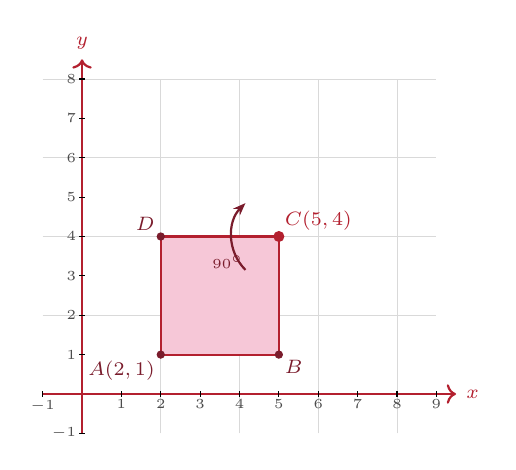
\begin{tikzpicture}[x=0.5cm,y=0.5cm]
\axg{-1}{-1}{9}{8}
\fill[pinkx!30] (2,1)--(5,1)--(5,4)--(2,4)--cycle;
\draw[redx,thick] (2,1)--(5,1)--(5,4)--(2,4)--cycle;
\draw[-{Stealth[length=1.6mm]},thick,maroon] ($(5,4)+(225:1.2)$) arc[start angle=225,end angle=135,radius=1.2];
\node[font=\tiny,maroon] at (3.7,3.35) {$90^\circ$};
\pnt{2}{1}{A(2,1)}{below left}\pnt{5}{1}{B}{below right}\pnt{2}{4}{D}{above left}
\fill[redx] (5,4) circle (2pt) node[above right,font=\scriptsize,inner sep=2pt]{$C(5,4)$};
\end{tikzpicture}}}{\pil{$(8,1)$}{$(2,7)$}{$(8,7)$}{$(-1,7)$}{$(5,-2)$}}
\soal{\gbr{Garis $2x+3y=6$ diputar $90^\circ$ berlawanan arah jarum jam dengan pusat $O$. Bayangan garis tersebut memotong sumbu-$x$ di titik \dots.}{%
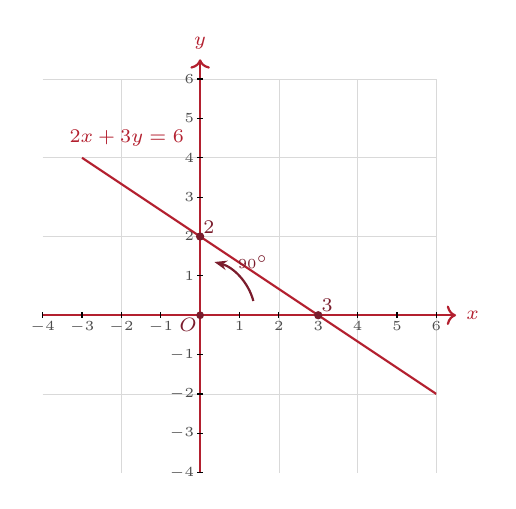
\begin{tikzpicture}[x=0.5cm,y=0.5cm]
\axg{-4}{-4}{6}{6}
\begin{scope}\clip (-4,-4) rectangle (6,6);\draw[thick,redx] (-3,4)--(6,-2);\end{scope}
\node[font=\scriptsize,redx,above right,inner sep=1pt] at (-3.4,4.2) {$2x+3y=6$};
\fill[maroon] (3,0) circle (1.5pt) node[above right,font=\scriptsize,inner sep=1pt]{$3$};
\fill[maroon] (0,2) circle (1.5pt) node[above right,font=\scriptsize,inner sep=1pt]{$2$};
\draw[-{Stealth[length=1.6mm]},thick,maroon] (15:1.4) arc[start angle=15,end angle=75,radius=1.4];
\node[font=\tiny,maroon] at (45:1.9) {$90^\circ$};
\fill[maroon] (0,0) circle (1.4pt) node[below left,font=\scriptsize,inner sep=1pt]{$O$};
\end{tikzpicture}}}{\pil{$(3,0)$}{$(2,0)$}{$(-3,0)$}{$(-2,0)$}{$(-6,0)$}}
\soal{\gbr{Segitiga $ABC$ pada gambar ditransformasikan oleh matriks $\begin{bmatrix}3&1\\-2&4\end{bmatrix}$, kemudian hasilnya didilatasi berpusat di $O$ dengan faktor $\frac12$. Luas bayangan akhir adalah \dots\ satuan luas.}{%
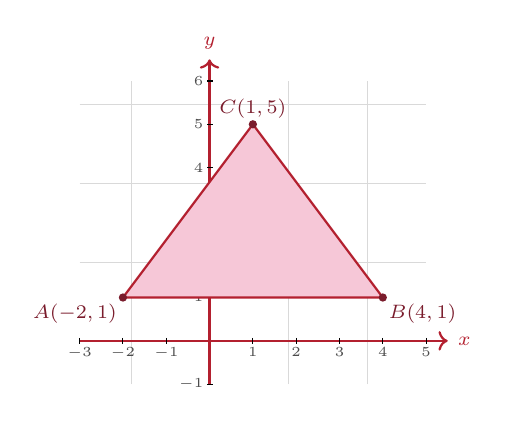
\begin{tikzpicture}[x=0.55cm,y=0.55cm]
\axg{-3}{-1}{5}{6}
\fill[pinkx!30] (-2,1)--(4,1)--(1,5)--cycle;
\draw[redx,thick] (-2,1)--(4,1)--(1,5)--cycle;
\pnt{-2}{1}{A(-2,1)}{below left}\pnt{4}{1}{B(4,1)}{below right}\pnt{1}{5}{C(1,5)}{above}
\end{tikzpicture}}}{\pil{$42$}{$84$}{$168$}{$21$}{$6$}}
\soal{Misalkan $T_1$ adalah refleksi terhadap sumbu-$x$ dan $T_2$ adalah rotasi $90^\circ$ berlawanan arah jarum jam berpusat di $O$. Tentukan benar atau salah setiap pernyataan berikut.}{\kat{$(T_2\circ T_1)(3,2)=(2,3)$.}{$(T_1\circ T_2)(3,2)=(2,3)$.}{$T_2\circ T_1$ ekuivalen dengan refleksi terhadap garis $y=x$.}{$T_1\circ T_2$ ekuivalen dengan refleksi terhadap garis $y=-x$.}}

\tingkat{Tingkat Sulit}{soal 11 sampai 15, setara UTBK}
\soal{\gbr{Pada layar kendali sebuah drone, posisi drone ditandai titik $P(1,5)$. Posisi tersebut dicerminkan terhadap garis $y=x+2$, kemudian bayangannya didilatasi berpusat di $C(2,-1)$ dengan faktor $-2$. Posisi akhir pada layar adalah \dots.}{%
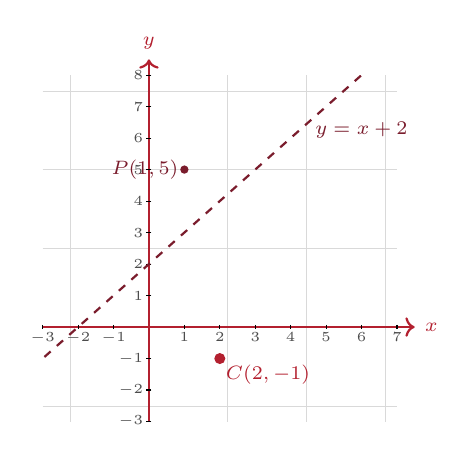
\begin{tikzpicture}[x=0.45cm,y=0.4cm]
\axg{-3}{-3}{7}{8}
\begin{scope}\clip (-3,-3) rectangle (7,8);\draw[dashed,maroon,thick] (-4,-2)--(7,9);\end{scope}
\node[font=\scriptsize,maroon,below right,inner sep=1pt] at (4.6,6.6) {$y=x+2$};
\pnt{1}{5}{P(1,5)}{left}
\fill[redx] (2,-1) circle (2pt) node[below right,font=\scriptsize,inner sep=2pt]{$C(2,-1)$};
\end{tikzpicture}}}{\pil{$(-8,-1)$}{$(-6,-6)$}{$(-4,-5)$}{$(4,7)$}{$(0,-9)$}}
\soal{\gbr{Parabola $y=x^2-4x+5$ pada gambar diputar $90^\circ$ berlawanan arah jarum jam dengan pusat $O$. Persamaan bayangannya adalah \dots.}{%
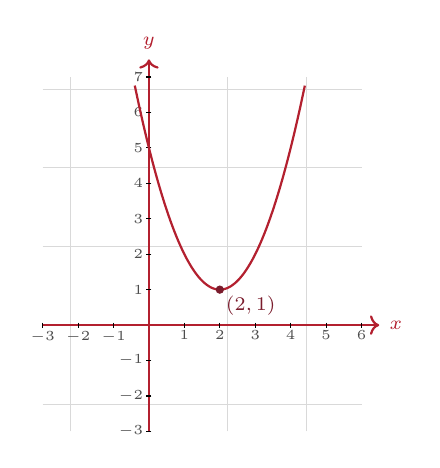
\begin{tikzpicture}[x=0.45cm,y=0.45cm]
\axg{-3}{-3}{6}{7}
\draw[thick,redx,domain=-0.4:4.4,smooth,samples=40] plot (\x,{\x*\x-4*\x+5});
\fill[maroon] (2,1) circle (1.5pt) node[below right,font=\scriptsize,inner sep=2pt]{$(2,1)$};
\end{tikzpicture}}}{\pilx{$x=y^2-4y+5$}{$x=y^2+4y+5$}{$x=-y^2+4y-5$}{$y=-x^2+4x-5$}{$x=-y^2-4y-5$}}
\soal{\gbr{Suatu dilatasi dengan faktor $3$ memetakan $A(2,1)$ ke $A'(-2,-5)$. Titik pusat dilatasi tidak diketahui. Bayangan titik $B(0,-1)$ oleh dilatasi yang sama adalah \dots.}{%
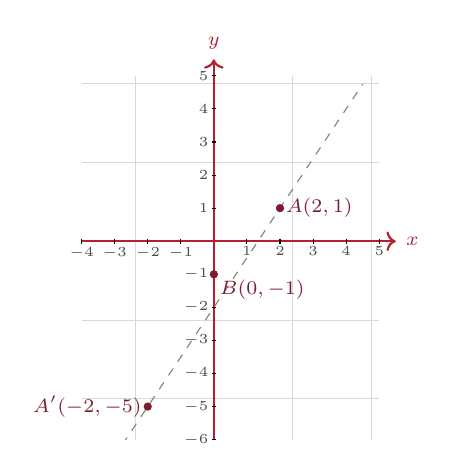
\begin{tikzpicture}[x=0.42cm,y=0.42cm]
\axg{-4}{-6}{5}{5}
\begin{scope}\clip (-4,-6) rectangle (5,5);\draw[dashed,gray] (-3.6,-7.4)--(4.5,4.75);\end{scope}
\pnt{2}{1}{A(2,1)}{right}\pnt{-2}{-5}{A'(-2,-5)}{left}\pnt{0}{-1}{B(0,-1)}{below right}
\end{tikzpicture}}}{\pil{$(0,-3)$}{$(0,1)$}{$(8,5)$}{$(-8,-11)$}{$(-4,-7)$}}
\soal{\gbr{Segitiga $ABC$ dengan $A(0,0)$, $B(3,0)$, $C(0,2)$ dipetakan ke segitiga $A'B'C'$ dengan $A'(4,2)$, $B'(1,2)$, $C'(4,0)$ (lihat gambar). Pilih \emph{semua} transformasi berikut yang memetakan $\triangle ABC$ tepat ke $\triangle A'B'C'$ dengan $A\to A'$, $B\to B'$, $C\to C'$.}{%
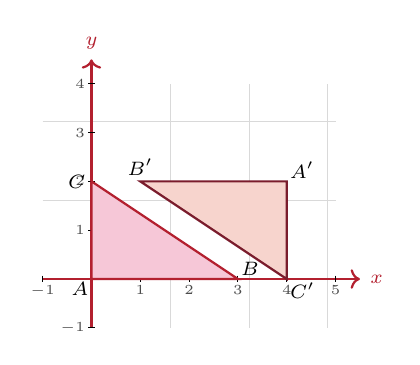
\begin{tikzpicture}[x=0.62cm,y=0.62cm]
\axg{-1}{-1}{5}{4}
\fill[pinkx!30] (0,0)--(3,0)--(0,2)--cycle;
\fill[salmon!35] (4,2)--(1,2)--(4,0)--cycle;
\draw[redx,thick] (0,0)--(3,0)--(0,2)--cycle;
\draw[maroon,thick] (4,2)--(1,2)--(4,0)--cycle;
\node[font=\scriptsize,below left,inner sep=1pt] at (0,0) {$A$};
\node[font=\scriptsize,above right,inner sep=1pt] at (3,0) {$B$};
\node[font=\scriptsize,left,inner sep=2pt] at (0,2) {$C$};
\node[font=\scriptsize,above right,inner sep=1pt] at (4,2) {$A'$};
\node[font=\scriptsize,above,inner sep=2pt] at (1,2) {$B'$};
\node[font=\scriptsize,below right,inner sep=1pt] at (4,0) {$C'$};
\end{tikzpicture}}}{\pilk{Rotasi $180^\circ$ berpusat di $(2,1)$.}{Dilatasi berpusat di $(2,1)$ dengan faktor $-1$.}{Refleksi terhadap garis $y=1$.}{Refleksi terhadap garis $y=1$ dilanjutkan refleksi terhadap garis $x=2$.}{Translasi oleh $\sm{4\\2}$.}}
\soal{\gbr{Persegi dengan panjang sisi $6$ cm diputar $45^\circ$ terhadap titik pusat persegi tersebut. Luas daerah irisan persegi semula dan bayangannya (daerah arsiran pada gambar) adalah \dots\ cm$^2$.}{%
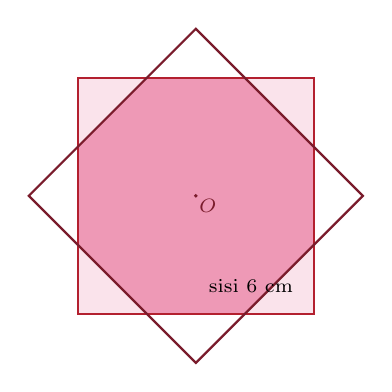
\begin{tikzpicture}[scale=0.5]
\fill[pinkx!15] (-3,-3) rectangle (3,3);
\begin{scope}\clip (-3,-3) rectangle (3,3);\fill[pinkx!55] (4.243,0)--(0,4.243)--(-4.243,0)--(0,-4.243)--cycle;\end{scope}
\draw[redx,thick] (-3,-3) rectangle (3,3);
\draw[maroon,thick] (4.243,0)--(0,4.243)--(-4.243,0)--(0,-4.243)--cycle;
\fill[maroon] (0,0) circle (1.4pt) node[below right,font=\scriptsize,inner sep=1pt]{$O$};
\node[font=\scriptsize] at (1.4,-2.3) {sisi $6$ cm};
\end{tikzpicture}}}{\pil{$36(\sqrt2-1)$}{$72(2-\sqrt2)$}{$72(\sqrt2-1)$}{$36\sqrt2$}{$72\sqrt2$}}

\tingkat{Tingkat HOTS}{soal 16 sampai 20, penalaran tingkat tinggi gaya TKA dan UTBK}
\soal{\gbr{Sebuah sungai lurus memiliki tepi atas pada garis $y=4$ dan tepi bawah pada garis $y=2$ (satuan km). Desa $A(1,10)$ berada di sebelah atas sungai dan desa $B(7,0)$ di sebelah bawah sungai. Pemerintah membangun satu jembatan lurus yang tegak lurus tepi sungai. Jalan dari $A$ ke jembatan dan dari jembatan ke $B$ berupa garis lurus. Panjang lintasan terpendek dari $A$ ke $B$ melalui jembatan adalah \dots\ km.}{%
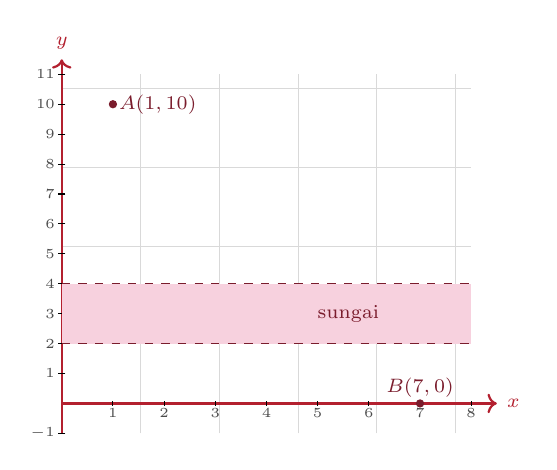
\begin{tikzpicture}[x=0.65cm,y=0.38cm]
\axg{0}{-1}{8}{11}
\fill[pinkx!25] (0,2) rectangle (8,4);
\draw[dashed,maroon] (0,2)--(8,2) (0,4)--(8,4);
\node[font=\scriptsize,maroon] at (5.6,3) {sungai};
\pnt{1}{10}{A(1,10)}{right}\pnt{7}{0}{B(7,0)}{above}
\end{tikzpicture}}}{\pil{$12$}{$10$}{$11$}{$14$}{$2\sqrt{34}$}}
\soal{\gbr{Suatu refleksi memetakan titik $A(0,5)$ ke $A'(4,3)$. Bayangan titik $B(5,5)$ oleh refleksi yang sama adalah \dots.}{%
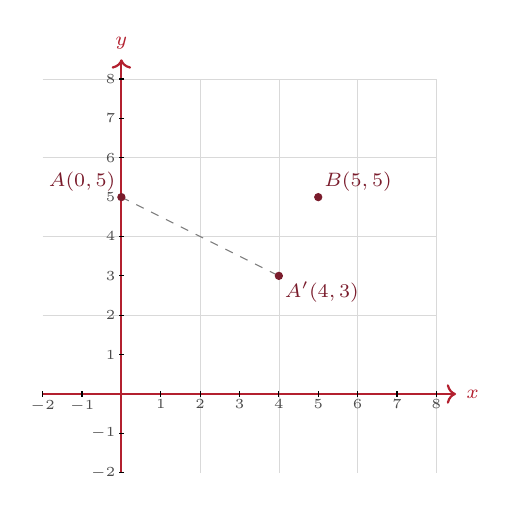
\begin{tikzpicture}[x=0.5cm,y=0.5cm]
\axg{-2}{-2}{8}{8}
\draw[dashed,gray] (0,5)--(4,3);
\pnt{0}{5}{A(0,5)}{above left}\pnt{4}{3}{A'(4,3)}{below right}\pnt{5}{5}{B(5,5)}{above right}
\end{tikzpicture}}}{\pil{$(3,6)$}{$(7,1)$}{$(5,-5)$}{$(-1,7)$}{$(1,7)$}}
\soal{Dilatasi $D_1$ berpusat di $P(1,2)$ dengan faktor $2$ dilanjutkan dilatasi $D_2$ berpusat di $Q(4,-1)$ dengan faktor $-1$. Komposisi $D_2\circ D_1$ ekuivalen dengan sebuah dilatasi tunggal. Pusat dilatasi tunggal tersebut adalah \dots.}{\pil{$(2,1)$}{$(3,0)$}{$\left(\dis\frac52,\frac12\right)$}{$(9,0)$}{$(-3,0)$}}

\Needspace{16\baselineskip}\par\vspace{0.75em}
\begin{tcolorbox}[colback=softbg,colframe=pinkx,boxrule=0.8pt,arc=3pt,left=7pt,right=7pt,top=4pt,bottom=4pt,title={\bfseries Stimulus untuk soal 19 dan 20},coltitle=white,fonttitle=\small]
\gbr{Sebuah aplikasi desain memiliki tiga tombol untuk mentransformasikan objek: tombol \textbf{R} memutar objek $90^\circ$ berlawanan arah jarum jam berpusat di $O$; tombol \textbf{F} mencerminkan objek terhadap garis $x=2$; tombol \textbf{G} menggeser objek oleh $\sm{3\\-1}$. Satu \emph{urutan} berarti menekan tombol R, F, G secara berturut-turut. Sebuah logo berbentuk segitiga $ABC$ dengan $A(1,1)$, $B(3,1)$, dan $C(1,2)$ (lihat gambar) diubah memakai urutan tersebut.}{%
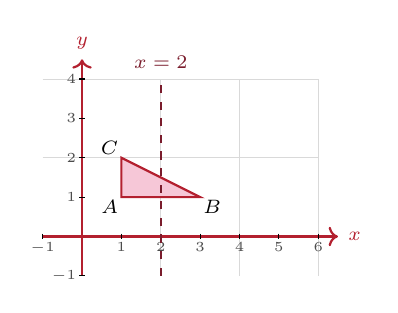
\begin{tikzpicture}[x=0.5cm,y=0.5cm]
\axg{-1}{-1}{6}{4}
\fill[pinkx!30] (1,1)--(3,1)--(1,2)--cycle;
\draw[redx,thick] (1,1)--(3,1)--(1,2)--cycle;
\draw[dashed,maroon,thick] (2,-1)--(2,4) node[above,font=\scriptsize]{$x=2$};
\node[font=\scriptsize,below left,inner sep=1pt] at (1,1) {$A$};
\node[font=\scriptsize,below right,inner sep=1pt] at (3,1) {$B$};
\node[font=\scriptsize,above left,inner sep=1pt] at (1,2) {$C$};
\end{tikzpicture}}
\end{tcolorbox}
\soal{Jika urutan R, F, G ditekan dua kali berturut-turut (enam tombol), koordinat bayangan akhir titik $B$ adalah \dots.}{\pil{$(8,2)$}{$(7,9)$}{$(9,7)$}{$(10,8)$}{$(12,0)$}}
\soal{Tentukan benar atau salah setiap pernyataan berikut.}{\kat{Luas bayangan segitiga $ABC$ setelah \emph{satu kali} urutan sama dengan luas semula.}{Urutan titik $A'\to B'\to C'$ pada bayangan (satu kali urutan) memiliki arah putaran yang berlawanan dengan arah $A\to B\to C$ semula.}{Terdapat sebuah titik yang posisinya tidak berubah setelah satu kali urutan.}{Setelah urutan ditekan dua kali berturut-turut, setiap titik pada logo tergeser oleh vektor yang sama, yaitu $\sm{6\\6}$.}}

% =====================================================================
\Needspace{16\baselineskip}
\bagian{B. Isian Singkat}{5 soal $\times$ 4 poin = 20 poin. Tuliskan hanya jawaban akhir.}

\tingkat{Tingkat Sedang}{soal 1 dan 2}
\soal{Titik $P(a,b)$ dicerminkan terhadap garis $y=-x$, kemudian bayangannya diputar $90^\circ$ berlawanan arah jarum jam dengan pusat $(1,1)$ sehingga menjadi titik $(-2,3)$. Nilai $a+b$ adalah \dots.}{\jwb}
\soal{\gbr{Persegi $ABCD$ dengan $A(1,1)$, $B(4,5)$, $C(8,2)$, dan $D(5,-2)$ didilatasi dengan pusat $P(0,5)$ dan faktor $-3$. Selisih luas bayangan dan luas persegi semula adalah \dots\ satuan luas.}{%
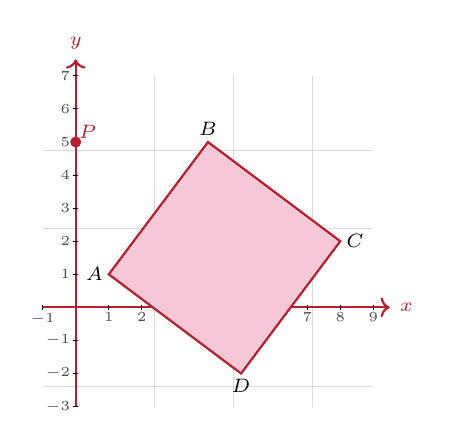
\begin{tikzpicture}[x=0.42cm,y=0.42cm]
\axg{-1}{-3}{9}{7}
\fill[pinkx!30] (1,1)--(4,5)--(8,2)--(5,-2)--cycle;
\draw[redx,thick] (1,1)--(4,5)--(8,2)--(5,-2)--cycle;
\node[font=\scriptsize,left,inner sep=2pt] at (1,1) {$A$};
\node[font=\scriptsize,above,inner sep=2pt] at (4,5) {$B$};
\node[font=\scriptsize,right,inner sep=2pt] at (8,2) {$C$};
\node[font=\scriptsize,below,inner sep=2pt] at (5,-2) {$D$};
\fill[redx] (0,5) circle (2pt) node[above right,font=\scriptsize,inner sep=1pt]{$P$};
\end{tikzpicture}}}{\jwb}

\tingkat{Tingkat Sulit}{soal 3 sampai 5}
\soal{Titik yang posisinya tidak berubah oleh transformasi ``rotasi $90^\circ$ berlawanan arah jarum jam berpusat di $O$ dilanjutkan translasi $\sm{4\\2}$'' adalah \dots.}{\jwb}
\soal{Persegi satuan dengan titik sudut $O(0,0)$, $P(1,0)$, $Q(1,1)$, dan $R(0,1)$ ditransformasikan oleh matriks $M=\begin{bmatrix}k&3\\2&k\end{bmatrix}$ sehingga menjadi sebuah jajargenjang berluas $5$ satuan luas. Pada bayangannya, urutan titik sudut $O\to P\to Q\to R$ yang semula berlawanan arah jarum jam berubah menjadi searah jarum jam. Nilai $k^2$ adalah \dots.}{\jwb}
\soal{Titik $P(5,2)$ diputar $90^\circ$ berlawanan arah jarum jam dengan pusat $C(1,-1)$. Bayangannya diputar lagi dengan pusat dan arah yang sama, begitu seterusnya sampai terjadi $2026$ kali rotasi. Koordinat posisi akhir titik $P$ adalah \dots.}{\jwb}

% =====================================================================
\Needspace{16\baselineskip}
\bagian{C. Uraian}{5 soal $\times$ 8 poin = 40 poin. Tuliskan langkah penyelesaian dengan lengkap.}

\tingkat{Tingkat Sedang}{soal 1 dan 2}
\soal{\gbr{Pada permainan blok susun, setiap kotak papan ditandai dengan koordinat pusatnya $(x,y)$. Sebuah blok berbentuk L menempati kotak $(2,6)$, $(3,6)$, $(4,6)$, dan $(4,7)$, dengan kotak $(3,6)$ sebagai poros. Pemain memberi tiga perintah berurutan: \textbf{R}: blok diputar $90^\circ$ searah jarum jam berpusat di poros $(3,6)$; \textbf{C}: blok dicerminkan terhadap garis $x=5$; \textbf{J}: blok digeser oleh $\sm{0\\-4}$.\par\smallskip
(a) Tentukan koordinat keempat kotak blok setelah perintah R.\par
(b) Tentukan koordinat keempat kotak setelah perintah C.\par
(c) Tentukan koordinat keempat kotak setelah perintah J, lalu periksa apakah blok tepat mengisi lubang berarsir putus-putus, yaitu kotak $(6,1)$, $(7,1)$, $(7,2)$, dan $(7,3)$.\par
(d) Jika pemain menjalankan J sebelum C (urutan R, J, C), apakah posisi akhir berubah? Jelaskan dengan rumus transformasinya.}{%
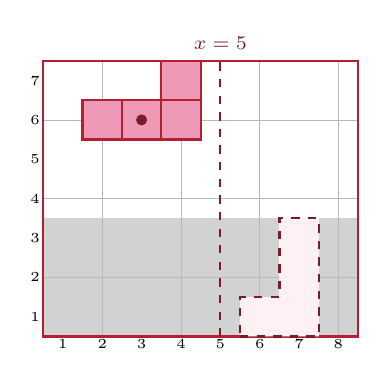
\begin{tikzpicture}[x=0.5cm,y=0.5cm]
\foreach \c in {1,...,5}{\foreach \r in {1,2,3}{\fill[gray!35] (\c-0.5,\r-0.5) rectangle (\c+0.5,\r+0.5);}}
\foreach \r in {2,3}{\fill[gray!35] (5.5,\r-0.5) rectangle (6.5,\r+0.5);}
\foreach \r in {1,2,3}{\fill[gray!35] (7.5,\r-0.5) rectangle (8.5,\r+0.5);}
\draw[gray!55,very thin] (0.5,0.5) grid (8.5,7.5);
\draw[redx,thick] (0.5,0.5) rectangle (8.5,7.5);
\draw[dashed,maroon,thick,fill=softbg] (5.5,0.5)--(7.5,0.5)--(7.5,3.5)--(6.5,3.5)--(6.5,1.5)--(5.5,1.5)--cycle;
\foreach \c/\r in {2/6,3/6,4/6,4/7}{\fill[pinkx!55] (\c-0.5,\r-0.5) rectangle (\c+0.5,\r+0.5);\draw[redx,thick] (\c-0.5,\r-0.5) rectangle (\c+0.5,\r+0.5);}
\fill[maroon] (3,6) circle (2pt);
\draw[dashed,maroon,thick] (5,0.5)--(5,7.5);
\node[font=\scriptsize,maroon] at (5,7.95) {$x=5$};
\foreach \c in {1,...,8}{\node[font=\tiny,below,inner sep=1pt] at (\c,0.5) {\c};}
\foreach \r in {1,...,7}{\node[font=\tiny,left,inner sep=1pt] at (0.5,\r) {\r};}
\end{tikzpicture}}}{\poin{8}}
\soal{\gbr{Sebuah proyektor yang lampunya berada di titik $P(1,2)$ memproyeksikan gambar segitiga $ABC$ dengan $A(2,3)$, $B(4,3)$, dan $C(3,5)$ ke layar. Proses ini dimodelkan sebagai dilatasi berpusat di $P$ dengan faktor $k=3$, dan bayangan segitiga ditulis $A'B'C'$.\par\smallskip
(a) Tentukan koordinat $A'$, $B'$, dan $C'$.\par
(b) Hitung luas dan keliling $\triangle A'B'C'$, lalu bandingkan dengan luas dan keliling $\triangle ABC$.\par
(c) Tentukan persamaan garis $AC$ dan garis $A'C'$. Apa hubungan kedua garis tersebut?\par
(d) Layar hanya dapat menampung titik dengan absis $x\le 8$ (garis putus-putus pada gambar). Jika pusat $P$ tetap, tentukan faktor skala $k>0$ terbesar agar seluruh bayangan tetap tampak pada layar.}{%
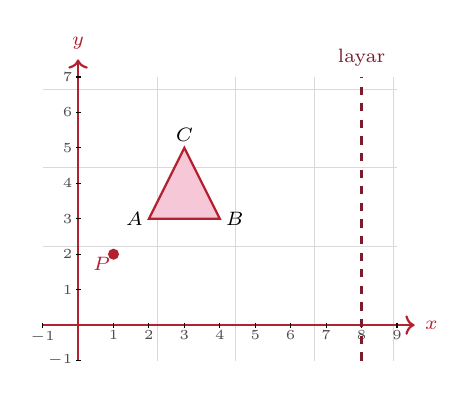
\begin{tikzpicture}[x=0.45cm,y=0.45cm]
\axg{-1}{-1}{9}{7}
\fill[pinkx!30] (2,3)--(4,3)--(3,5)--cycle;
\draw[redx,thick] (2,3)--(4,3)--(3,5)--cycle;
\draw[dashed,maroon,thick] (8,-1)--(8,7) node[above,font=\scriptsize]{layar};
\node[font=\scriptsize,left,inner sep=2pt] at (2,3) {$A$};
\node[font=\scriptsize,right,inner sep=2pt] at (4,3) {$B$};
\node[font=\scriptsize,above,inner sep=2pt] at (3,5) {$C$};
\fill[redx] (1,2) circle (2pt) node[below left,font=\scriptsize,inner sep=1pt]{$P$};
\end{tikzpicture}}}{\poin{8}}

\tingkat{Tingkat Sulit}{soal 3 dan 4}
\soal{\gbr{Ruas garis $AB$ dengan $A(1,1)$ dan $B(5,1)$ dipetakan oleh sebuah rotasi menjadi ruas $A'B'$ dengan $A'(4,0)$ dan $B'(4,4)$ (lihat gambar). Pusat rotasi $C$ tidak diketahui.\par\smallskip
(a) Tunjukkan bahwa $AB=A'B'$, lalu jelaskan mengapa pusat rotasi harus berjarak sama dari $A$ dan $A'$, serta dari $B$ dan $B'$.\par
(b) Tentukan persamaan sumbu ruas $AA'$ dan sumbu ruas $BB'$, lalu tentukan koordinat pusat rotasi $C$.\par
(c) Tunjukkan bahwa $\angle ACA'=90^\circ$, lalu tentukan arah rotasinya (searah atau berlawanan arah jarum jam).\par
(d) Tentukan bayangan titik $D(1,5)$ oleh rotasi tersebut.}{%
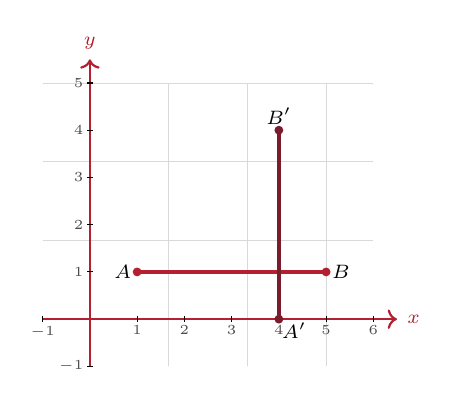
\begin{tikzpicture}[x=0.6cm,y=0.6cm]
\axg{-1}{-1}{6}{5}
\draw[redx,very thick] (1,1)--(5,1);
\draw[maroon,very thick] (4,0)--(4,4);
\node[font=\scriptsize,left,inner sep=2pt] at (1,1) {$A$};
\node[font=\scriptsize,right,inner sep=2pt] at (5,1) {$B$};
\node[font=\scriptsize,below right,inner sep=1pt] at (4,0) {$A'$};
\node[font=\scriptsize,above,inner sep=2pt] at (4,4) {$B'$};
\fill[redx] (1,1) circle (1.6pt) (5,1) circle (1.6pt);
\fill[maroon] (4,0) circle (1.6pt) (4,4) circle (1.6pt);
\end{tikzpicture}}}{\poin{8}}
\soal{\gbr{Transformasi $T$ dengan matriks $M=\begin{bmatrix}a&b\\c&d\end{bmatrix}$ memetakan titik $P(1,1)$ ke $P'(2,3)$ dan titik $Q(2,-1)$ ke $Q'(7,0)$ (lihat gambar: segitiga $OPQ$ dan bayangannya $OP'Q'$).\par\smallskip
(a) Tentukan matriks $M$.\par
(b) Hitung $\det M$, kemudian tentukan luas $\triangle OP'Q'$ dengan dua cara: memakai faktor $|\det M|$ dan memakai koordinat titik sudutnya.\par
(c) Tentukan titik $R$ yang bayangannya adalah $R'(7,14)$.\par
(d) Tentukan persamaan bayangan garis $x+2y=7$ oleh $T$. Apa yang dapat disimpulkan tentang arah garis bayangan tersebut?}{%
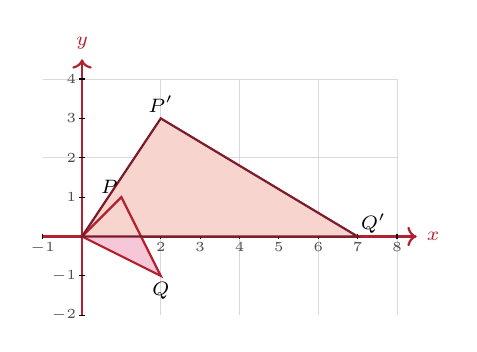
\begin{tikzpicture}[x=0.5cm,y=0.5cm]
\axg{-1}{-2}{8}{4}
\fill[pinkx!30] (0,0)--(1,1)--(2,-1)--cycle;
\fill[salmon!35] (0,0)--(2,3)--(7,0)--cycle;
\draw[redx,thick] (0,0)--(1,1)--(2,-1)--cycle;
\draw[maroon,thick] (0,0)--(2,3)--(7,0)--cycle;
\node[font=\scriptsize,above left,inner sep=1pt] at (1,1) {$P$};
\node[font=\scriptsize,below,inner sep=2pt] at (2,-1) {$Q$};
\node[font=\scriptsize,above,inner sep=2pt] at (2,3) {$P'$};
\node[font=\scriptsize,above right,inner sep=1pt] at (7,0) {$Q'$};
\end{tikzpicture}}}{\poin{8}}

\tingkat{Tingkat HOTS}{soal 5}
\soal{\gbr{Meja biliar berbentuk persegi panjang dengan sudut-sudut $(0,0)$, $(8,0)$, $(8,4)$, dan $(0,4)$ (satuan dm). Bola putih berada di $A(2,1)$ dan bola sasaran di $B(6,1)$. Pemain memukul bola putih sehingga bola memantul lebih dahulu pada dinding atas ($y=4$) di titik $P$, kemudian memantul pada dinding kanan ($x=8$) di titik $Q$, lalu mengenai bola sasaran $B$. Pada setiap dinding, sudut datang sama dengan sudut pantul.\par\smallskip
(a) Cerminkan $B$ terhadap dinding kanan menjadi $B_1$, lalu cerminkan $B_1$ terhadap dinding atas menjadi $B_2$. Tentukan koordinat $B_1$ dan $B_2$.\par
(b) Jelaskan mengapa panjang lintasan $A\to P\to Q\to B$ sama dengan $AB_2$, lalu hitung panjang lintasan tersebut.\par
(c) Tentukan koordinat $P$ dan $Q$, dan periksa bahwa keduanya benar-benar berada pada dinding meja.\par
(d) Titik $B_2$ juga dapat diperoleh dari $B$ oleh satu rotasi $180^\circ$. Tentukan pusat rotasinya dan jelaskan alasannya. Kemudian hitung panjang lintasan jika bola hanya memantul satu kali pada dinding atas, dan bandingkan dengan hasil (b).}{%
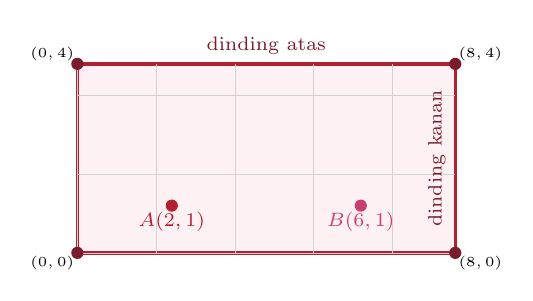
\begin{tikzpicture}[x=0.6cm,y=0.6cm]
\fill[softbg] (0,0) rectangle (8,4);
\draw[redx,very thick] (0,0) rectangle (8,4);
\draw[gray!35,very thin] (0,0) grid (8,4);
\foreach \p in {(0,0),(8,0),(8,4),(0,4)}{\fill[maroon] \p circle (2.2pt);}
\node[font=\tiny,below left,inner sep=1pt] at (0,0) {$(0,0)$};
\node[font=\tiny,below right,inner sep=1pt] at (8,0) {$(8,0)$};
\node[font=\tiny,above right,inner sep=1pt] at (8,4) {$(8,4)$};
\node[font=\tiny,above left,inner sep=1pt] at (0,4) {$(0,4)$};
\node[font=\scriptsize,maroon,above] at (4,4) {dinding atas};
\node[font=\scriptsize,maroon,rotate=90,above] at (8,2) {dinding kanan};
\fill[redx] (2,1) circle (2.2pt) node[below,font=\scriptsize,inner sep=2pt]{$A(2,1)$};
\fill[pinkx!90!black] (6,1) circle (2.2pt) node[below,font=\scriptsize,inner sep=2pt]{$B(6,1)$};
\end{tikzpicture}}}{\poin{8}}

% =====================================================================
\newpage
\bagian{Kunci Jawaban dan Pembahasan Singkat}{Untuk guru dan pembahasan mandiri}
\par\vspace{0.6em}{\bfseries\color{redx}Kunci Pilihan Ganda}\par\vspace{0.3em}
\small
\begin{tabularx}{\linewidth}{@{}*{10}{>{\centering\arraybackslash}X}@{}}\hline \textbf{1} & \textbf{2} & \textbf{3} & \textbf{4} & \textbf{5} & \textbf{6} & \textbf{7} & \textbf{8} & \textbf{9} & \textbf{10}\\ \hline D & C & E & A & {\scriptsize A,B,D,E} & B & B & D & A & {\scriptsize B,S,B,B}\\ \hline\end{tabularx}\\[6pt]
\begin{tabularx}{\linewidth}{@{}*{10}{>{\centering\arraybackslash}X}@{}}\hline \textbf{11} & \textbf{12} & \textbf{13} & \textbf{14} & \textbf{15} & \textbf{16} & \textbf{17} & \textbf{18} & \textbf{19} & \textbf{20}\\ \hline E & C & D & {\scriptsize A,B,D} & C & A & E & B & C & {\scriptsize B,B,S,B}\\ \hline\end{tabularx}
\par\vspace{0.8em}{\bfseries\color{redx}\normalsize Pembahasan Pilihan Ganda}\par\vspace{0.2em}
\small\begin{enumerate}[leftmargin=2em,itemsep=2pt,topsep=2pt]
\item[\textbf{1.}] \textbf{(D)} Vektor translasi $T=A'-A=(5-(-2),\,1-6)=(7,-5)$. Maka $B'=(3+7,\,-4-5)=(10,-9)$. (Jebakan A: memakai $A-A'$, sehingga arah translasi terbalik.)
\item[\textbf{2.}] \textbf{(C)} Pada refleksi terhadap $y=k$: $(x,y)\mapsto(x,\,2k-y)$. Untuk $C(-1,6)$ dan $k=2$: $C'=(-1,\,4-6)=(-1,-2)$. (Jebakan A: memakai sumbu-$x$; jebakan B: memakai $k-y$ tanpa dikali $2$.)
\item[\textbf{3.}] \textbf{(E)} Rotasi $270^\circ$ berlawanan arah jarum jam sama dengan rotasi $90^\circ$ searah jarum jam: $(x,y)\mapsto(y,-x)$. Maka $Q'=(5,\,3)$. (Jebakan A: rotasi $90^\circ$ berlawanan arah jarum jam; jebakan B: rotasi $180^\circ$.)
\item[\textbf{4.}] \textbf{(A)} Faktor dilatasi $k=\frac{-12}{3}=\frac{8}{-2}=-4$. Maka $B'=(-4)(-1,5)=(4,-20)$.
\item[\textbf{5.}] \textbf{(A, B, D, E)} Translasi, rotasi, dan refleksi adalah isometri (jarak dan luas tetap). Dilatasi mengalikan luas dengan $k^2$; untuk $k=-1$ berlaku $k^2=1$ sehingga luas tetap. Pilihan C salah karena luasnya menjadi $4$ kali.
\item[\textbf{6.}] \textbf{(B)} Misalkan $P(a,b)$: $3a-2b=0$ dan $a+4b=14$, sehingga $a=2$ dan $b=3$. Refleksi terhadap $y=-x$: $(x,y)\mapsto(-y,-x)$, jadi $(-3,-2)$. (Jebakan A: refleksi terhadap $y=x$.)
\item[\textbf{7.}] \textbf{(B)} $A-C=(-3,-3)$. Rotasi $90^\circ$ searah jarum jam: $(x,y)\mapsto(y,-x)$ memberi $(-3,3)$. Maka $A'=C+(-3,3)=(2,7)$. (Jebakan A: rotasi berlawanan arah jarum jam memberi $(8,1)$.) Perhatikan pula bahwa $B'=(2,4)=D$.
\item[\textbf{8.}] \textbf{(D)} Rotasi $90^\circ$ berlawanan arah jarum jam: $x'=-y$, $y'=x$, sehingga $x=y'$ dan $y=-x'$. Substitusi: $2y'-3x'=6$. Memotong sumbu-$x$ saat $y=0$: $-3x=6\Rightarrow x=-2$. Titik $(-2,0)$ (bayangan dari titik $(0,2)$). (Jebakan B: rotasi searah jarum jam.)
\item[\textbf{9}.] \textbf{(A)} Luas $\triangle ABC=\frac12\cdot6\cdot4=12$. $\det=3\cdot4-1\cdot(-2)=14$, sehingga luas setelah matriks $=14\cdot12=168$. Dilatasi faktor $\frac12$ mengalikan luas dengan $\left(\frac12\right)^2=\frac14$: $168\cdot\frac14=42$. (Jebakan B: faktor $\frac12$ tidak dikuadratkan.)
\item[\textbf{10.}] \textbf{(B, S, B, B)} (1) $T_1(3,2)=(3,-2)$, lalu $T_2(3,-2)=(2,3)$: \emph{benar}. (2) $T_2(3,2)=(-2,3)$, lalu $T_1(-2,3)=(-2,-3)\neq(2,3)$: \emph{salah}. (3) $(x,y)\to(x,-y)\to(y,x)$: itu refleksi terhadap $y=x$, \emph{benar}. (4) $(x,y)\to(-y,x)\to(-y,-x)$: itu refleksi terhadap $y=-x$, \emph{benar}. Jadi $T_1\circ T_2\neq T_2\circ T_1$.
\item[\textbf{11.}] \textbf{(E)} Refleksi terhadap $y=x+2$: geser garis ke $y=x$ (turun $2$), tukar koordinat, lalu geser naik $2$, sehingga $(x,y)\mapsto(y-2,\,x+2)$. $P(1,5)\mapsto(3,3)$. Dilatasi $[C(2,-1),-2]$: $C+(-2)\big((3,3)-C\big)=(2,-1)+(-2)(1,4)=(0,-9)$. (Jebakan C: menganggap cermin $y=x$.)
\item[\textbf{12.}] \textbf{(C)} Rotasi $90^\circ$ berlawanan arah jarum jam: $x'=-y$, $y'=x$, sehingga $x=y'$ dan $y=-x'$. Substitusi ke $y=x^2-4x+5$: $-x'=y'^2-4y'+5$, yaitu $x=-y^2+4y-5$. Puncak $(2,1)$ menjadi $(-1,2)$, cocok dengan $x=-(2)^2+4(2)-5=-1$. (B adalah hasil rotasi searah jarum jam; A adalah refleksi terhadap $y=x$.)
\item[\textbf{13.}] \textbf{(D)} Pusat $C$ memenuhi $A'=C+3(A-C)=3A-2C$, sehingga $C=\frac{3A-A'}{2}=\frac{(6+2,\;3+5)}{2}=(4,4)$. Maka $B'=3B-2C=(0-8,\,-3-8)=(-8,-11)$. (Jebakan A: menganggap pusat di $O$.)
\item[\textbf{14.}] \textbf{(A, B, D)} Pusat $(2,1)$ adalah titik tengah $AA'$, $BB'$, dan $CC'$, jadi rotasi $180^\circ$ di $(2,1)$ memetakan $A\to A'$, $B\to B'$, $C\to C'$ (A benar). Dilatasi faktor $-1$ dengan pusat sama adalah transformasi yang sama (B benar). Refleksi $y=1$ saja memberi $A\mapsto(0,2)$, salah (C). Refleksi terhadap $y=1$ lalu $x=2$ memberi $(x,y)\mapsto(4-x,\,2-y)$, yaitu rotasi $180^\circ$ di $(2,1)$ (D benar). Translasi $\sm{4\\2}$ memetakan $B$ ke $(7,2)\neq B'$ (E salah).
\item[\textbf{15.}] \textbf{(C)} Irisan kedua persegi adalah segidelapan beraturan dengan apotema $3$ cm (setengah sisi persegi). Luas $=8\cdot3^2\cdot\tan22{,}5^\circ=72(\sqrt2-1)$ cm$^2$ (sekitar $29{,}8$). (Jebakan B: $72(2-\sqrt2)$ adalah luas \emph{gabungan}.)
\item[\textbf{16.}] \textbf{(A)} Geser $B$ ke atas sejauh lebar sungai (dua satuan) menjadi $B^*(7,2)$. Panjang $QB$ sama dengan $PB^*$ untuk jembatan $PQ$ tegak lurus, sehingga lintasan terpendek memenuhi $AP+PB^*\ge AB^*=\sqrt{6^2+8^2}=10$. Tambahkan panjang jembatan $2$: total $12$ km. Jembatan berada di $x=5{,}5$: $AP=7{,}5$ dan $QB=2{,}5$. (Jebakan E: $AB=2\sqrt{34}\approx11{,}7$ tidak dapat dicapai karena jembatan harus tegak lurus tepi sungai.)
\item[\textbf{17.}] \textbf{(E)} Cermin adalah sumbu ruas $AA'$: titik tengah $(2,4)$, gradien $AA'=-\frac12$, sehingga gradien cermin $=2$ dan persamaannya $y=2x$. Kaki tegak lurus $B(5,5)$ pada cermin adalah $(3,6)$. Maka $B'=2(3,6)-(5,5)=(1,7)$. (Jebakan A: kaki tegak lurus; jebakan B: refleksi terhadap $y=x$.)
\item[\textbf{18.}] \textbf{(B)} $D_1(X)=P+2(X-P)=2X-P$ dan $D_2(Y)=Q-(Y-Q)=2Q-Y$. Komposisi: $D_2(D_1(X))=-2X+P+2Q$, yaitu dilatasi dengan faktor $-2$. Titik tetapnya memenuhi $X=-2X+P+2Q\Rightarrow X=\frac{P+2Q}{3}=\frac{(1+8,\;2-2)}{3}=(3,0)$.
\item[\textbf{19.}] \textbf{(C)} Satu urutan: $R:(x,y)\mapsto(-y,x)$, $F:(x,y)\mapsto(4-x,y)$, $G:(x,y)\mapsto(x+3,y-1)$. Gabungan $T(x,y)=(y+7,\,x-1)$. Maka $T(3,1)=(8,2)$ dan $T(8,2)=(9,7)$. Cek: $T^2(x,y)=(x+6,\,y+6)$, sehingga $B(3,1)\mapsto(9,7)$. (Jebakan A: hanya satu kali urutan.)
\item[\textbf{20.}] \textbf{(B, B, S, B)} (1) $T$ adalah isometri, luas tetap: \emph{benar}. (2) $A'(8,0)$, $B'(8,2)$, $C'(9,0)$ berputar searah jarum jam, sedangkan $A,B,C$ berlawanan arah jarum jam; bagian linear $T$ adalah $\sm{0&1\\1&0}$ dengan determinan $-1$: \emph{benar}. (3) Titik tetap memerlukan $x=y+7$ dan $y=x-1$, yang memberi $0=6$ (tidak ada solusi): \emph{salah}. (4) $T^2(x,y)=(x+6,y+6)$: \emph{benar}. $T$ berupa refleksi geser (glide reflection).
\end{enumerate}
\par\Needspace{6\baselineskip}\vspace{0.6em}{\bfseries\color{redx}\normalsize Pembahasan Isian Singkat}\par\vspace{0.2em}
\small\begin{enumerate}[leftmargin=2em,itemsep=2pt,topsep=2pt]
\item[\textbf{1.}] \textbf{Jawaban: $-7$.} Refleksi terhadap $y=-x$: $(a,b)\mapsto(-b,-a)$. Rotasi $90^\circ$ berlawanan arah jarum jam berpusat $(1,1)$: $(x,y)\mapsto(2-y,\,x)$, sehingga $(-b,-a)\mapsto(2+a,\,-b)=(-2,3)$. Jadi $a=-4$, $b=-3$, dan $a+b=-7$.
\item[\textbf{2.}] \textbf{Jawaban: $200$.} Sisi $AB=\sqrt{3^2+4^2}=5$, sehingga luas semula $25$. Dilatasi faktor $-3$ mengalikan luas dengan $(-3)^2=9$: $225$. Selisih $=225-25=200$.
\item[\textbf{3.}] \textbf{Jawaban: $(1,3)$.} Transformasinya $(x,y)\mapsto(-y+4,\;x+2)$. Titik tetap: $x=-y+4$ dan $y=x+2$, sehingga $x=-x-2+4\Rightarrow x=1$ dan $y=3$. Cek: $(1,3)\to(-3,1)\to(1,3)$.
\item[\textbf{4.}] \textbf{Jawaban: $1$.} Luas bayangan $=|\det M|\cdot1=|k^2-6|=5$, sehingga $k^2=11$ atau $k^2=1$. Orientasi berbalik berarti $\det M<0$, yaitu $k^2<6$. Jadi $k^2=1$ (dan $\det M=-5$).
\item[\textbf{5.}] \textbf{Jawaban: $(-3,-4)$.} Empat rotasi $90^\circ$ sama dengan satu putaran penuh, dan $2026=4\cdot506+2$. Jadi hasilnya sama dengan dua rotasi, yaitu $180^\circ$: $P'=2C-P=(2-5,\,-2-2)=(-3,-4)$.
\end{enumerate}
\par\Needspace{8\baselineskip}\vspace{0.6em}{\bfseries\color{redx}\normalsize Pembahasan dan Pedoman Penskoran Uraian}\par\vspace{0.2em}
\small\begin{enumerate}[leftmargin=2em,itemsep=3pt,topsep=2pt]
\item[\textbf{1.}] (a) $R:(x,y)\mapsto(3+(y-6),\;6-(x-3))=(y-3,\;9-x)$. Kotak menjadi $(3,7)$, $(3,6)$, $(3,5)$, $(4,5)$. (b) $C:(x,y)\mapsto(10-x,y)$. Kotak menjadi $(7,7)$, $(7,6)$, $(7,5)$, $(6,5)$. (c) $J:(x,y)\mapsto(x,y-4)$. Kotak menjadi $(7,3)$, $(7,2)$, $(7,1)$, $(6,1)$. Keempatnya sama dengan kotak lubang, jadi blok tepat mengisi lubang. (d) Urutan R, J, C: $(x,y)\to(x,y-4)\to(10-x,\,y-4)$. Urutan R, C, J: $(x,y)\to(10-x,y)\to(10-x,\,y-4)$. Hasilnya sama, karena refleksi terhadap garis tegak hanya mengubah absis sedangkan translasi vertikal hanya mengubah ordinat. \\ \textit{Penskoran: (a) 2 poin; (b) 2 poin; (c) 2 poin (koordinat 1, kesimpulan 1); (d) 2 poin.}
\item[\textbf{2.}] (a) $P'=P+3(X-P)$: $A'=(1,2)+3(1,1)=(4,5)$; $B'=(1,2)+3(3,1)=(10,5)$; $C'=(1,2)+3(2,3)=(7,11)$. (b) $L_{ABC}=\frac12\cdot2\cdot2=2$ dan $L_{A'B'C'}=\frac12\cdot6\cdot6=18$, yaitu $9=3^2$ kali. Keliling $ABC=2+2\sqrt5$ dan keliling $A'B'C'=6+6\sqrt5$, yaitu $3$ kali. (c) Gradien $AC=\frac{5-3}{3-2}=2$: $y=2x-1$. Gradien $A'C'=\frac{11-5}{7-4}=2$: $y=2x-3$. Kedua garis sejajar (dilatasi memetakan garis ke garis yang sejajar). (d) Absis bayangan: $x'=1+k(x-1)$. Absis terbesar ada pada $B$: $1+3k\le8\Rightarrow k\le\frac73$. Jadi $k_{\max}=\frac73$. \\ \textit{Penskoran: (a) 2 poin; (b) 2 poin (luas 1, keliling 1); (c) 2 poin; (d) 2 poin.}
\item[\textbf{3.}] (a) $AB=4$ dan $A'B'=4$. Rotasi mempertahankan jarak ke pusatnya, sehingga $CA=CA'$ dan $CB=CB'$; titik $C$ berada pada sumbu $AA'$ dan sumbu $BB'$. (b) $AA'$: titik tengah $\left(\frac52,\frac12\right)$, gradien $-\frac13$, sumbu: $y=3x-7$. $BB'$: titik tengah $\left(\frac92,\frac52\right)$, gradien $-3$, sumbu: $x=3y-3$. Substitusi: $x=3(3x-7)-3\Rightarrow x=3$, sehingga $y=2$. Pusat $C(3,2)$. (c) $\overrightarrow{CA}=(-2,-1)$ dan $\overrightarrow{CA'}=(1,-2)$: hasil kali titik $=-2+2=0$, jadi $\angle ACA'=90^\circ$. Hasil kali silang $(-2)(-2)-(-1)(1)=5>0$, jadi putaran dari $CA$ ke $CA'$ berlawanan arah jarum jam. (d) $D-C=(-2,3)\mapsto(-3,-2)$, sehingga $D'=(3,2)+(-3,-2)=(0,0)$. \\ \textit{Penskoran: (a) 2 poin; (b) 2 poin (sumbu 1, titik $C$ 1); (c) 2 poin (sudut 1, arah 1); (d) 2 poin.}
\item[\textbf{4.}] (a) Dari $a+b=2$ dan $2a-b=7$: $a=3$, $b=-1$. Dari $c+d=3$ dan $2c-d=0$: $c=1$, $d=2$. Jadi $M=\begin{bmatrix}3&-1\\1&2\end{bmatrix}$. (b) $\det M=6+1=7$. Luas $\triangle OPQ=\frac12|1\cdot(-1)-1\cdot2|=\frac32$. Cara 1: $L'=7\cdot\frac32=\frac{21}{2}$. Cara 2: $\triangle OP'Q'$ dengan $O(0,0)$, $P'(2,3)$, $Q'(7,0)$ memiliki luas $\frac12|2\cdot0-3\cdot7|=\frac{21}{2}$. Keduanya sama. (c) $M^{-1}=\frac17\begin{bmatrix}2&1\\-1&3\end{bmatrix}$, sehingga $R=\frac17(14+14,\;-7+42)=(4,5)$. Cek: $M(4,5)=(12-5,\,4+10)=(7,14)$. (d) $x=\frac{2x'+y'}{7}$ dan $y=\frac{-x'+3y'}{7}$. Maka $x+2y=\frac{2x'+y'-2x'+6y'}{7}=y'$, sehingga bayangannya $y=7$. Garis bayangan mendatar (sejajar sumbu-$x$), meskipun garis semula miring. \\ \textit{Penskoran: (a) 2 poin; (b) 2 poin (determinan 0,5, dua cara masing-masing 0,75); (c) 2 poin; (d) 2 poin (persamaan 1,5, kesimpulan 0,5).}
\item[\textbf{5.}] (a) $B_1=(16-6,\,1)=(10,1)$ dan $B_2=(10,\,8-1)=(10,7)$. (b) Panjang $QB=QB_1$ karena $Q$ pada dinding kanan, dan $PB_1=PB_2$ karena $P$ pada dinding atas. Pantulan sama dengan meneruskan lintasan lurus ke bayangan sasaran, sehingga lintasan setelah ``dilurus'kan'' adalah ruas $AB_2$. Panjangnya $\sqrt{(10-2)^2+(7-1)^2}=10$ dm. (c) Garis $AB_2$: $y-1=\frac34(x-2)$. Pada $y=4$: $x=6$, jadi $P(6,4)$ (benar pada dinding atas, $0<6<8$). Pada $x=8$: $y=\frac{11}{2}$, yang merupakan bayangan $Q$ terhadap $y=4$, sehingga $Q=\left(8,\,8-\frac{11}{2}\right)=\left(8,\frac52\right)$ (benar pada dinding kanan, $0<\frac52<4$). Cek: $AP=5$, $PQ=\frac52$, $QB=\frac52$, total $10$. (d) Dinding atas dan dinding kanan tegak lurus dan berpotongan di $(8,4)$. Komposisi dua refleksi terhadap garis yang saling tegak lurus adalah rotasi $180^\circ$ di titik potong: $B\mapsto(16-6,\;8-1)=(10,7)=B_2$. Jika hanya memantul pada dinding atas: $B^*=(6,7)$, panjang lintasan $AB^*=\sqrt{4^2+6^2}=2\sqrt{13}\approx7{,}2$ dm, lebih pendek sekitar $2{,}8$ dm daripada $10$ dm karena tidak ada pantulan tambahan. \\ \textit{Penskoran: (a) 2 poin; (b) 2 poin (alasan 1, panjang 1); (c) 2 poin ($P$ 0,75, $Q$ 0,75, pemeriksaan 0,5); (d) 2 poin (pusat dan alasan 1, perbandingan 1).}
\end{enumerate}
\end{document}
